\documentclass[11pt, a4paper]{article} % (NON MODIFIABLE)

%% Packages utilisés 
% (MODIFIABLE : des packages peuvent être ajoutés)
\usepackage[french]{babel}
\usepackage[utf8]{inputenc}
\usepackage[T1]{fontenc}
\usepackage[svgnames]{xcolor}
\usepackage{graphicx}
\usepackage{amsmath,amssymb,amsthm,amscd}
\usepackage{tabularx}
\usepackage{hyperref}
\usepackage{url}
\usepackage{geometry}
\usepackage{lscape}
\usepackage{pdfpages}
\usepackage{color}
\usepackage{float}

\usepackage{listings}


\geometry{hmargin=15mm,vmargin=20mm}

%% Environnement de "théorèmes"
% (MODIFIABLE)
\newtheorem{defin}{Définition}
\newtheorem{prop}{Proposition}
\newtheorem{thm}{Théorème}
\newtheorem{cor}{Corollaire}
\newtheorem{lem}{Lemme}
\newtheorem{nota}{Notation}
\newtheorem{rem}{Remarque}
\newtheorem{conj}{Conjecture}
\newtheorem{nb}{N.B.}
\let\oldtabular=\tabular
\def\tabular{\small\oldtabular}

%% Taille relative tolérée d'un objet flottant sur une page
% (MODIFIABLE)
\renewcommand{\floatpagefraction}{0.95}

%%%%%%%%%%%%%%%%%%%%%%%%%%%%%%%%%%%%%%%%%%%%%%%%%%%%%%%%%%%%%%%%%%%%%%%%%%%%%%%%
%% DÉBUT DU DOCUMENT
%%%%%%%%%%%%%%%%%%%%%%%%%%%%%%%%%%%%%%%%%%%%%%%%%%%%%%%%%%%%%%%%%%%%%%%%%%%%%%%%

\begin{document}

%%%%%%%%%%%%%%%%%%%%%%%%%%
% Première de couverture %
%%%%%%%%%%%%%%%%%%%%%%%%%%

\thispagestyle{empty}
\begin{center}
  {\LARGE UNIVERSITÉ D'ÉVRY -- VAL D'ESSONNE}
  \vskip 3mm
  {\LARGE Département d'informatique}\\
  \vskip 3mm
  \begin{figure}[h]
    \begin{center}
      
\includegraphics[scale=1]{logoUEVE.png}
		\end{center}
  \end{figure}
  \vskip 0cm
  {\LARGE Processus concurrents et temporisés}\\
  \vskip 3mm
  2nd année de Master informatique\\
  parcours CILS\\  
	\vskip 1cm
  Soutenu par\\
  \vskip 3mm {\LARGE {\bf Valentin COTTE, Vianney TOUCHARD}} 
  \vskip 3mm le 18 janvier 2019 
  \vfill {\huge {\bf Projet M2 : Modélisation et analyse d'automates temporisés avec UPPAAL et de réseaux de Petri temporels avec TINA}} \vfill
	\vskip 3mm
	\emph{Encadrant}\\
  Hanna KLAUDEL \\
  \vskip 3cm Année universitaire 2018-2019
\end{center}

\clearpage

%%%%%%%%%%%%%%%%%%%%%%
% Table des matières %
%%%%%%%%%%%%%%%%%%%%%%

\hrule\medskip

\begin{center}
  \tableofcontents
\end{center}

\medskip\hrule\bigskip\bigskip

%%%%%%%%%%%%%
% Sections %
%%%%%%%%%%%%%
\section{Introduction}
\label{sec:Intro}

L'objectif de ce projet est de modéliser un problème donné sous forme d'automates temporisés et réseaux de Petri, puis d'analyser et modifier ces modèles afin de répondre à 3 questions.\\
\\
On rappelle le système à modéliser:\\

\textit{Alice se rend à l'université en train (cela prend entre 20 et 30 min) ou en bus, ce qui est de 15 min plus rapide, mais elle doit marcher pendant 5 min pour rejoindre l'arrêt de bus.\\
\\
Bob vient à l'université en voiture (entre 30 et 40 min) ou en train (50 min). Il a besoin de 5 à 10 min pour garer sa voiture et autant pour passer de l'arrêt de tram à l'université.\\
\\
Claire habite à proximité et vient à l'université à pied (entre 15 et 20 min) ou à vélo (5 min), mais dans ce cas, elle doit laisser son vélo dans un parking distant ce qui prend 5 min à 10 min pour rejoindre l'université.\\}
\\
On ajoute à ce système les contraintes suivantes:\\
\textit{Ce matin, Alice est partie de chez elle entre 7h50 et 8h. Bob est arrivé à l'université entre 8h10 et 8h20. De plus, Claire est partie 10 à 20 minutes après Alice et Bob.\\}
\\
Et enfin, voici les 3 questions auxquelles il faut répondre:
\begin{itemize}
    \item 1) Les contraintes temporelles figurant dans ce scénario sont-elles consistantes?
    \item 2) Est-il possible qu'Alice ait pris le bus et Claire ait utilisé le vélo?
    \item 3) Dans quelle plage horaire Bob a pu partir?
\end{itemize}

\clearpage

\section{Automates Temporisés (UPPAAL)}
\label{sec:UPPAAL}
La première étape est de convenir de la modélisation du système. Dans l'annexe~\ref{A}, les automates temporisés permettent une modélisation assez proche de l'énoncé. \\
Nous commençons par définir une horloge globale qui représente l'heure (en nombre de minutes écoulées depuis minuit). Chaque personnage est représenté par un automate et les places sont les différents endroits où peuvent être Alice, Bob et Claire. Les contraintes énoncées sont directement ajoutées sur les arcs et les places comme des invariants et des conditions. 

\subsection{Question 1}
\label{sub:UPPAALQ1}
De par la modélisation choisie, les contraintes sont satisfiables si une exécution amène A., B. et C. à l'université.\\
Pour obtenir une réponse du vérifieur, on lui soumet le prédicat négatif exprimant << A., B. ou C. n'est pas à l'université >>. Le vérifieur infirme et soumet un contre-exemple : les contraintes peuvent donc être satisfaites, elles sont consistantes.

\begin{figure}[h]
    \begin{flushleft}
      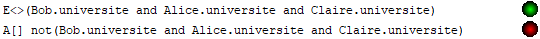
\includegraphics[scale=0.60]{captures/uppaalQ1.png}
    \end{flushleft}
\end{figure}


\subsection{Question 2}
\label{sub:UPPAALQ2}
Nous avons encore une fois recours à la négation de la proposition pour que UPPAAL fournisse un contre-exemple.\\
Le contre-exemple s'exprime << (Alice a pris le bus => Claire n'a pas utilisé le vélo) et (Claire a utilisé le vélo => Alice n'a pas pris le bus) >>. Plus formellement, nous avons la proposition équivalente : non(il existe un chemin tel que A.b et C.v) = pour tout chemin, Non(A.b) ou non(C.v)\\
Pour exprimer correctement cette contrainte, il faut garder à l'esprit qu'on ne peut pas se contenter de vérifier l'existence d'un état où Alice.bus et Claire.velo sont actifs, car ces états pourraient être actifs à des moments différents et que la condition soit tout de même validée. Ainsi, nous avons recours à des variables drapeaux qui restent activés.\\
Cette précaution prise, le prouveur nous donne un contre-exemple où les contraintes sont respectées et où Alice utilise le bus et Claire le vélo.

\begin{figure}[h]
    \begin{flushleft}
      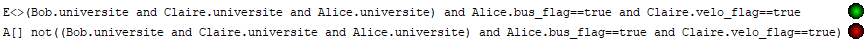
\includegraphics[scale=0.60]{captures/uppaalQ2.png}
    \end{flushleft}
\end{figure}

\subsection{Question 3}
\label{sub:UPPAALQ3}
Pour cette question, nous nous trouvons obligés de procéder par tâtonnements en cherchant les valeurs (supérieure et inférieure) de la plage horaire cherchée.\\
Cette plage horaire correspond à celle que nous avons trouvée à la main : Bob doit partir entre 7h10 et 7h45 pour que l'énoncé soit respecté.\\
Cela fait, on valide les horaires vérifiant la formule <<Bob est parti en dehors de la plage horaire => les contraintes de l'énoncé ne seront pas satisfaites>>

\begin{figure}[h]
    \begin{flushleft}
      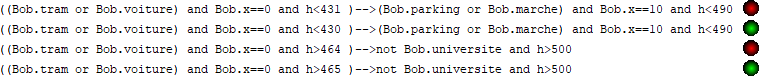
\includegraphics[scale=0.60]{captures/uppaalQ3.png}
      
\includegraphics[scale=0.50]{captures/uppaalQ3bis.png}
    \end{flushleft}
\end{figure}

\clearpage

\section{Réseaux de Petri (TINA)}
\label{sec:TINA}
Pour cette seconde partie, nous avons une modélisation du système tout aussi proche de l'énoncé. Cependant, contrairement aux automates temporisés, les réseaux de Petri en annexe~\ref{B} sont indépendants des contraintes de l'énoncé. C'est à l'aide de réseaux <<observateurs>> que nous allons faire respecter les contraintes dans des requêtes LTL.\\
Les différents agents sont donc Alice, Bob et Claire qui vont parcourir chacun un réseau différent simulant leur trajet jusqu'à l'université, ainsi que deux observateurs: un pour renseigner l'heure actuelle et un autre pour chronométrer depuis combien de temps Bob et Alice sont partis de chez eux (ce dernier est uniquement utile pour la contrainte du départ de Claire).

\subsection{Question 1}
\label{sub:TINAQ1}

Tout comme l'on fait nos prédécesseurs dans l'article \cite{berthomieu2006reseaux}, nous avons fait calculé par TINA un graphe de classe du réseau de l'annexe~\ref{B} afin de vérifier la satisfiabilité de formules LTL.\\
Pour montrer la consistance des contraintes, il faut prouver l'existence d'une exécution dans laquelle Alice, Bob et Claire vont à l'université tout en respectant toutes les contraintes de l'énoncé.\\
Il s'agit de vérifier la satisfiabilité de la formule signifiant qu'il n'existe pas de telle exécution:\\
\\
$\lnot( \ \lozenge \ (depart\_alice \ \wedge \ 7h50\_8h00) \\
\wedge \ \lozenge \ (arrivee\_bob \ \wedge \  8h10\_8h20) \\
\wedge \  \lozenge \ (depart\_claire \ \wedge \ 10\_20) \\
\wedge \ \lozenge \ (univ\_alice \ \wedge \ univ\_bob \ \wedge \ univ\_claire))$
\\
\\
Avec le model checker $selt$, nous trouvons que cette formule est fausse. Pour le prouver, il nous renvoie une trace contre-exemple, soit une trace qui respecte toutes les contraintes et donc prouve qu'elles sont consistantes.

\subsection{Question 2}
\label{sub:TINAQ2}
Ici, contrairement à la situation pour les automates temporisés, pas besoin de variables : le chemin complet est considéré. Nous rajoutons aux contraintes précédentes la proposition voulue, et un contre-exemple est trouvé.\\
\\
$\lnot( \ \lozenge \ (univ\_bob \ \wedge \ univ\_alice \ \wedge \ univ\_claire) \\
\wedge \ \lozenge \ (depart\_alice \ \wedge \ 7h50\_8h00) \\
\wedge \ \lozenge \ (arrivee\_bob \ \wedge \ 8h10\_8h20) \\
\wedge \ \lozenge \ (depart\_claire \ \wedge \ 10\_20) \\
\wedge \ \lozenge \ alice\_bus \ \wedge \ \lozenge \ claire\_velo)$

\subsection{Question 3}
\label{sub:TINAQ3}
Pour cette question, on rajoute une branche à l'observateur qui nous permet de vérifier la présence dans une plage précise. Encore une fois, nous approchons les valeurs par le haut et par le bas. Une fois la plage trouvée, on peut vérifier qu'un départ en dehors de celle-ci ne permet pas aux contraintes d'être satisfaites.\\
Pour cela, on a donc fabriqué 3 réseaux identiques à l'annexe~\ref{B} mais avec un observateur différent. Avec chacun d'eux, nous avons testé une série de formules LTL pour trouver la plage horaire du départ de Bob.\\

\clearpage

\begin{figure}[h]
    \begin{flushleft}
      \hspace*{-10mm}
      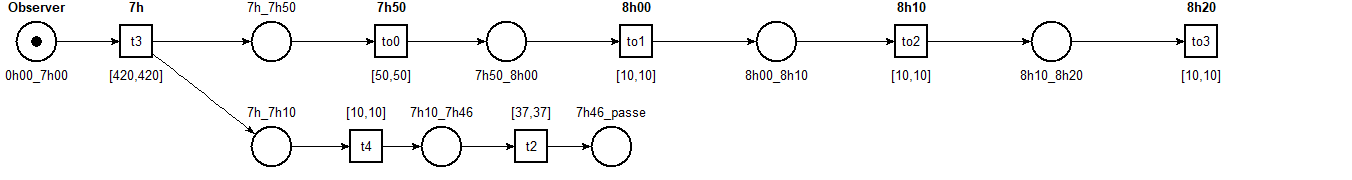
\includegraphics[scale=0.6]{captures/q3_borne_inferieure.PNG}
    \end{flushleft}
\end{figure}

\noindent
$\lnot( \ \lozenge \ (univ\_bob \ \wedge \ univ\_alice \ \wedge \ univ\_claire) \\
\wedge \ \lozenge \ (depart\_alice \ \wedge \ 7h50\_8h00) \\
\wedge \ \lozenge \ (arrivee\_bob \ \wedge \ 8h10\_8h20) \\
\wedge \ \lozenge \ (depart\_claire \ \wedge \ 10\_20) \\
\wedge \ \lozenge \ (depart\_bob \ \wedge \ (0h00\_7h00 \ \vee \ 7h\_7h10)))\\$
\\
La formule renvoie un contre-exemple, ce qui nous donne un départ déjà possible à 7h10.\\

\begin{figure}[h]
    \begin{flushleft}
      \hspace*{-10mm}
      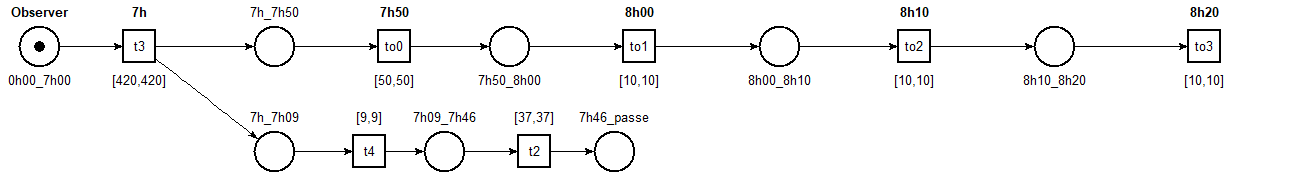
\includegraphics[scale=0.6]{captures/q3_synthese.PNG}
    \end{flushleft}
\end{figure}

\noindent
$\lnot( \ \lozenge \ (univ\_bob \ \wedge \ univ\_alice \ \wedge \ univ\_claire) \\
\wedge \ \lozenge \ (depart\_alice \ \wedge \ 7h50\_8h00) \\
\wedge \ \lozenge \ (arrivee\_bob \ \wedge \ 8h10\_8h20) \\
\wedge \ \lozenge \ (depart\_claire \ \wedge \ 10\_20) \\
\wedge \ \lozenge \ (depart\_bob \ \wedge \ (7h45\_passe)))\\$
\\
La formule renvoie un contre-exemple, ce qui nous donne un départ encore possible à 7h45.\\

\begin{figure}[h]
    \begin{flushleft}
      \hspace*{-10mm}
      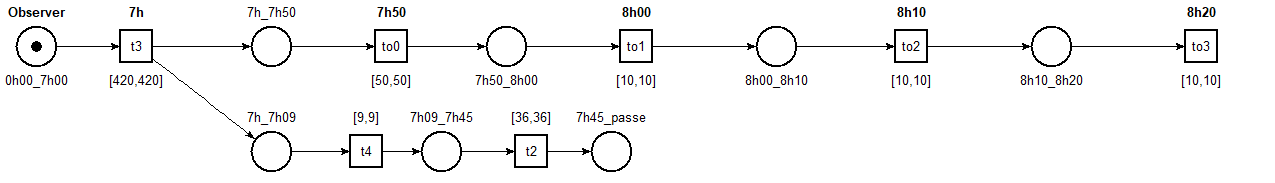
\includegraphics[scale=0.6]{captures/q3_borne_superieure.PNG}
    \end{flushleft}
\end{figure}
\noindent
$\lnot( \ \lozenge \ (univ\_bob \ \wedge \ univ\_alice \ \wedge \ univ\_claire) \\
\wedge \ \lozenge \ (depart\_alice \ \wedge \ 7h50\_8h00) \\
\wedge \ \lozenge \ (arrivee\_bob \ \wedge \ 8h10\_8h20) \\
\wedge \ \lozenge \ (depart\_claire \ \wedge \ 10\_20) \\
\wedge \ \lozenge \ (depart\_bob \ \wedge \ (0h00\_7h00 \ \vee \ 7h\_7h09)))\\$
\\
La proposition est vraie, ce qui donne un départ impossible avant 7h10.\\
\\

\clearpage

\noindent
$\lnot( \ \lozenge \ (univ\_bob \ \wedge \ univ\_alice \ \wedge \ univ\_claire) \\
\wedge \ \lozenge \ (depart\_alice \ \wedge \ 7h50\_8h00) \\
\wedge \ \lozenge \ (arrivee\_bob \ \wedge \ 8h10\_8h20) \\
\wedge \ \lozenge \ (depart\_claire \ \wedge \ 10\_20) \\
\wedge \ \lozenge \ (depart\_bob \ \wedge \ (7h46\_passe)))\\$
\\
La proposition est vraie, ce qui donne un départ impossible après 7h46.\\
\\
On peut donc confirmer l'impossibilité de partir hors de cette tranche horaire avec:\\
$\lnot( \ \lozenge \ (univ\_bob \ \wedge \ univ\_alice \ \wedge \ univ\_claire) \\
\wedge \ \lozenge \ (depart\_alice \ \wedge \ 7h50\_8h00) \\
\wedge \ \lozenge \ (arrivee\_bob \ \wedge \ 8h10\_8h20) \\
\wedge \ \lozenge \ (depart\_claire \ \wedge \ 10\_20) \\
\wedge \ \lozenge \ (depart\_bob \ \wedge \ \lnot 7h09\_7h46))\\$
\\
La formule est évaluée à vrai, donc la plage horaire est de 7h10 à 7h45.\\
Une façon plus élégante aurait été de définir cette plage comme un intervalle ouvert plutôt qu'en rajoutant une minute.



%%%%%%%%%%%%%%%%%
% Bibliographie %
%%%%%%%%%%%%%%%%%	

\nocite{*}
\bibliographystyle{alpha}
\bibliography{biblio}

\clearpage

%%%%%%%%%%%%
% Annexes %
%%%%%%%%%%%
\newgeometry{hmargin=5mm,vmargin=5mm, rmargin=0mm}

\newpage
\appendix
\setcounter{page}{1}
\renewcommand{\thepage}{\roman{page}}


\begin{landscape}

\section{Annexe}
\label{A}
   \begin{figure}[h]
    \begin{center}
      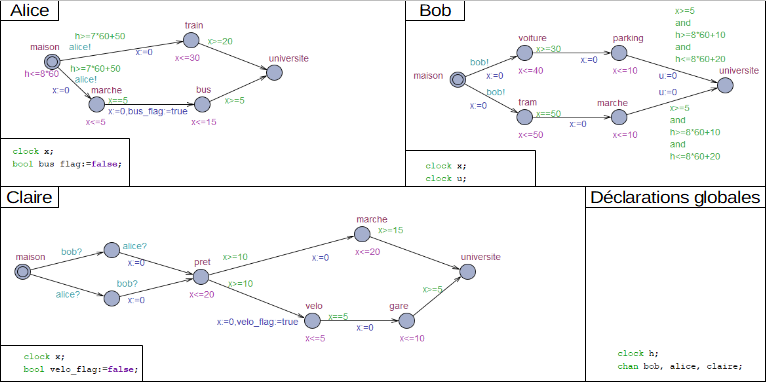
\includegraphics[scale=1]{captures/Automates.png}
      \caption{Modélisation du système en automates temporisés avec les contraintes}
    \end{center}
\end{figure}

\clearpage

\section{Annexe}
\label{B}
   \begin{figure}[h]
    \begin{center}
      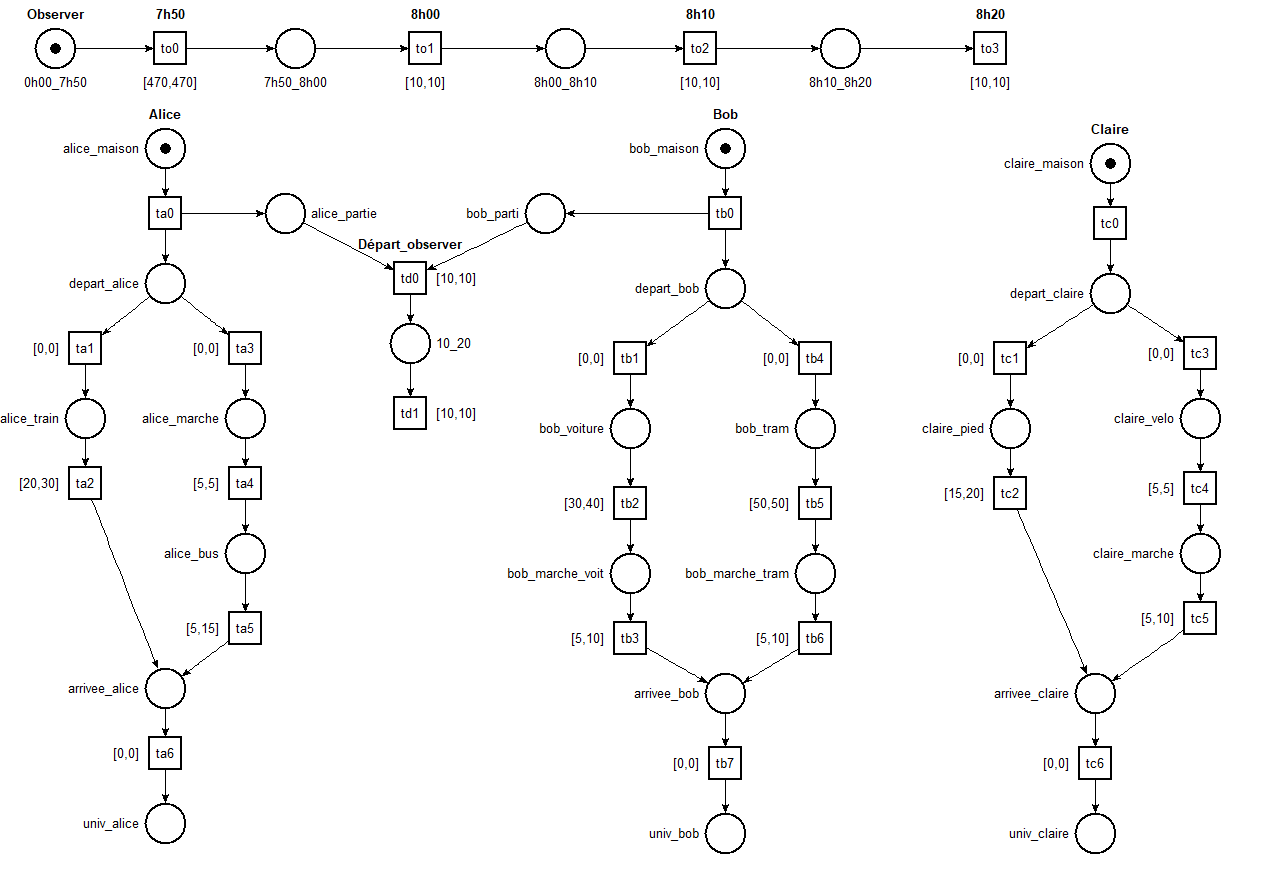
\includegraphics[scale=0.62]{captures/petri1.PNG}
      \caption{Modélisation du système en réseaux de Petri temporels avec les observateurs}
    \end{center}
\end{figure}
      
\end{landscape}

\end{document}
